\newif\ifshowsolutions
\showsolutionstrue
\documentclass{article}
\usepackage{listings}
\usepackage{amsmath}
\usepackage{subfig}
\usepackage{amsthm}
\usepackage{amsmath}
\usepackage{amssymb}
\usepackage{graphicx}
\usepackage{mdwlist}
\usepackage{geometry}
\usepackage{titlesec}
\usepackage{palatino}
\usepackage{mathrsfs}
\usepackage{fancyhdr}
\usepackage{paralist}
\usepackage{todonotes}
\usepackage{tikz}
\usepackage{float} % Place figures where you ACTUALLY want it
\usepackage{comment} % A hack to toggle sections
\usepackage{ifthen}
\usepackage{mdframed}
\usepackage{verbatim}
\usepackage{listings}
\usepackage{bbm}
\usepackage{upquote} % Prevents backticks replacing single-quotes in verbatim
\usepackage[strings]{underscore}
\usepackage[colorlinks=true]{hyperref}
\usetikzlibrary{positioning,shapes,backgrounds}

\geometry{margin=1in}
\geometry{headheight=2in}
\geometry{top=2in}

\setlength{\marginparwidth}{2.15cm}
\setlength{\parindent}{0em}
\setlength{\parskip}{0.6\baselineskip}

\rhead{}
\lhead{}

% Spacing settings.
\titlespacing\section{0pt}{12pt plus 2pt minus 2pt}{0pt plus 2pt minus 2pt}
\titlespacing\subsection{0pt}{12pt plus 4pt minus 2pt}{0pt plus 2pt minus 2pt}
\titlespacing\subsubsection{0pt}{12pt plus 4pt minus 2pt}{0pt plus 2pt minus 2pt}
\renewcommand{\baselinestretch}{1.15}

% Shortcuts for commonly used operators.
\newcommand{\E}{\mathbb{E}}
\newcommand{\Var}{\operatorname{Var}}
\newcommand{\Cov}{\operatorname{Cov}}
\newcommand{\Bias}{\operatorname{Bias}}
\DeclareMathOperator{\argmin}{arg\,min}
\DeclareMathOperator{\argmax}{arg\,max}

% Do not number subsections and below.
\setcounter{secnumdepth}{1}

% Custom format subsection.
\titleformat*{\subsection}{\large\bfseries}

% Set up the problem environment.
\newcounter{problem}[section]
\newenvironment{problem}[1][]
  {\begingroup
    \setlength{\parskip}{0em}
    \refstepcounter{problem}\par\addvspace{1em}\textbf{Problem~\Alph{problem}\!
    \ifthenelse{\equal{#1}{}}{}{ [#1 points]}:}
  \endgroup}

% Set up the subproblem environment.
\newcounter{subproblem}[problem]
\newenvironment{subproblem}[1][]
  {\begingroup
    \setlength{\parskip}{0em}
    \refstepcounter{subproblem}\par\medskip\textbf{\roman{subproblem}.\!
    \ifthenelse{\equal{#1}{}}{}{ [#1 points]:}}
  \endgroup}

% Set up the teachers and materials commands.
\newcommand\teachers[1]
  {\begingroup
    \setlength{\parskip}{0em}
    \vspace{0.3em} \textit{\hspace*{2em} TAs responsible: #1} \par
  \endgroup}
\newcommand\materials[1]
  {\begingroup
    \setlength{\parskip}{0em}
    \textit{\hspace*{2em} Relevant materials: #1} \par \vspace{1em}
  \endgroup}

% Set up the hint environment.
\newenvironment{hint}[1][]
  {\begin{em}\textbf{Hint: }}
  {\end{em}}


% Set up the solution environment.
\ifshowsolutions
  \newenvironment{solution}[1][]
    {\par\medskip \begin{mdframed}\textbf{Solution~\Alph{problem}#1:} \begin{em}}
    {\end{em}\medskip\end{mdframed}\medskip}
  \newenvironment{subsolution}[1][]
    {\par\medskip \begin{mdframed}\textbf{Solution~\Alph{problem}#1.\roman{subproblem}:} \begin{em}}
    {\end{em}\medskip\end{mdframed}\medskip}
\else
  \excludecomment{solution}
  \excludecomment{subsolution}
\fi




%%%%%%%%%%%%%%%%%%%%%%%%%%%%%%
% HEADER
%%%%%%%%%%%%%%%%%%%%%%%%%%%%%%

\chead{
  {\vbox{
      \vspace{2mm}
      \large
      Machine Learning \& Data Mining \hfill
      Caltech CS/CNS/EE 155 \hfill \\[1pt]
      Set 5\hfill
      February 2022\\
    }
  }
}

\newcommand{\Tr}{\operatornamewithlimits{Tr}}

\begin{document}
\pagestyle{fancy}



%%%%%%%%%%%%%%%%%%%%%%%%%%%%%%
% POLICIES
%%%%%%%%%%%%%%%%%%%%%%%%%%%%%%


% \section*{Policies}
% \begin{itemize}
% 	\item Due 9 PM PST, February $16^\text{th}$ on Gradescope. 
% 	\item You are free to collaborate on all of the problems, subject to the collaboration policy stated in the syllabus.
% 	\item If you have trouble with this homework, it may be an indication that you should drop the class.
% 	\item In this course, we will be using Google Colab for code submissions. You will need a Google account.
% \end{itemize}

% \section*{Submission Instructions}

% \begin{itemize}
% 	\item Submit your report as a single .pdf file to Gradescope (entry code 7426YK), under "Set 5 Report". 
% 	\item In the report, \textbf{include any images generated by your code} along with your answers to the questions.
% 	\item Submit your code by \textbf{sharing a link in your report} to your Google Colab notebook for each problem (see naming instructions below). Make sure to set sharing permissions to at least "Anyone with the link can view". \textbf{Links that can not be run by TAs will not be counted as turned in.} Check your links in an incognito window before submitting to be sure. 
% 	\item For instructions specifically pertaining to the Gradescope submission process, see \url{https://www.gradescope.com/get_started#student-submission}.
  
% \end{itemize}


% \section*{Google Colab Instructions}

% For each notebook, you need to save a copy to your drive.

% \begin{enumerate}
% 	\item Open the github preview of the notebook, and click the icon to open the colab preview.
% 	\item On the colab preview, go to File $\rightarrow$ Save a copy in Drive.
% 	\item Edit your file name to “lastname_firstname_originaltitle”, e.g.”yue_yisong_3_notebook_part1.ipynb”
% \end{enumerate}


% \newpage

Homework submitted using 3 late hours. I have 45 late hours remaining.

\section{SVD and PCA [35 Points]}
\materials{Lectures 10, 11}

\problem[3] Let $X$ be a $N \times N$ matrix. For the singular value decomposition (SVD) $X = U \Sigma V^T$, show that the columns of $U$ are the principal components of $X$. What relationship exists between the singular values of $X$ and the eigenvalues of $XX^T$?

\begin{solution}
    The solution to PCA is $U$ such that $X X^T =  U \Lambda U^T$.
    \begin{align*}
        X X^T &= U \Sigma V^T (U \Sigma V^T)^T\\
        &= U \Sigma V^T V \Sigma^T U^T\\
        &= U \Sigma \Sigma^T U^T && \text{since $V$ is orthogonal}\\
        &= U \Sigma^2 U^T && \text{since $\Sigma$ is a diagonal matrix}
    \end{align*}
    Since $\Sigma$ is a diagonal matrix with the singular values of $X$, $\Sigma^2$ is a diagonal matrix that satisifies $X X^T = U \Lambda U^T$ with $\Lambda = \Sigma^2$, since $U$ is orthogonal in both the singular value decomposition and the solution to PCA. Since $\Lambda$ is a diagonal matrix that contains the eigenvalues of $X$, the singular values of $X$ are the square roots of the eigenvalues of $X X^T$.
\end{solution}

\problem[4] Provide both an intuitive explanation and a mathematical justification for why the eigenvalues of the PCA of $X$ (or rather $XX^T$) are non-negative. Such matrices are called positive semi-definite and possess many other useful properties.

\begin{solution}
    We know that the eigenvalue
    \[
        \lambda_j = \sum_{i=1}^N (u_j^T x_i)^2
    \]
    which can also be interpreted as the variation along the axis $u_j$. The variation of a variable must be non-negative, so the eigenvalues in the PCA of $X$ are non-negative. Mathematically, since the eigenvalues of $X X^T$ are the squares of the singular values of $X$ ($\sigma$), they must be $\geq 0$, since the square of any real number is non-negative.
\end{solution}

\newpage

\problem[5] In calculating the Frobenius and trace matrix norms, we claimed that the trace is invariant under cyclic permutations (i.e., Tr($ABC$) = Tr($BCA$) = Tr($CAB$)). Prove that this holds for any number of square matrices.

\textit{Hint}: First prove that the identity holds for two matrices and then generalize. Recall that Tr$(AB) = \sum_{i=1}^{N}(AB)_{ii}$. Can you find a way to expand $(AB)_{ii}$ in terms of another sum?

\begin{solution}
    We can produce any cyclic permutation of the product $A_1 A_2 ... A_n$ by swapping 2 subproducts. Let the desired permutation be $A_i A_{i+1} ... A_n A_1 ... A_{i-1}$. Then, let $A' = A_i A_{i+1} ... A_n$ and $B' = A_1 ... A_{i-1}$. If we can show that $\Tr(A' B') = \Tr{(B' A')}$, then we have shown that $\Tr({A_1 A_2 ... A_n}) = \Tr({A_1 ... A_{i-1}})$ for any arbitrary cyclic permutation of an arbitrary length product of matrices.

    To show that $\Tr({A B}) = \Tr({B A})$, we use the given definition.
    \begin{align*}
        \Tr({A B}) &= \sum_{i=1}^N (AB)_{ii}\\
        &= \sum_{i=1}^N \sum_{j=1}^N A_{ij} B_{ji}\\
        &= \sum_{j=1}^N \sum_{i=1}^N B_{ji} A_{ij}\\
        &= \sum_{j=1}^N (B A)_{jj}\\
        &= \Tr({B A})
    \end{align*}
    Thus, the trace is invariant under cyclic permutation.
\end{solution}

\newpage

\problem[3] Outside of learning, the SVD is commonly used for data compression. Instead of storing a full $N \times N$ matrix $X$ with SVD $X = U\Sigma V^T$, we store a truncated SVD consisting of the $k$ largest singular values of $\Sigma$ and the corresponding columns of $U$ and $V$. One can prove that the SVD is the best rank-$k$ approximation of $X$, though we will not do so here. Thus, this approximation can often re-create the matrix well even for low $k$. Compared to the $N^2$ values needed to store $X$, how many values do we need to store a truncated SVD with $k$ singular values? For what values of $k$ is storing the truncated SVD more efficient than storing the whole matrix?

\textit{Hint}: For the diagonal matrix $\Sigma$, do we have to store every entry?

\begin{solution}
    In the matrix $U$, we must store $k N$ entries from the first $k$ columns, since these are multiplied by the first $k$ largest singular values. In the matrix $V$, we must store $k N$ entries from the first $k$ columns as well. We must also store $k$ values from $\Sigma$, which are the largest singular values. Since $\Sigma$ is a diagonal matrix, to store $k$ singular values, we only need to store $k$ values along the diagonal, since all other values are 0. Thus, in total we must store $2 k N + k$ values.

    For $N^2 > 2k N + k$ (less values stored using SVD method), we need $k < \frac{N^2}{2N + 1}$.
\end{solution}

\newpage

\subsection{Dimensions \& Orthogonality} In class, we claimed that a matrix $X$ of size $D \times N$ can be decomposed into $U\Sigma V^T$, where $U$ and $V$ are orthogonal and $\Sigma$ is a diagonal matrix. This is a slight simplification of the truth. In fact, the singular value decomposition gives an orthogonal matrix $U$ of size $D \times D$, an orthogonal matrix $V$ of size $N \times N$, and a rectangular diagonal matrix $\Sigma$ of size $D \times N$, where $\Sigma$ only has non-zero values on entries $(\Sigma)_{ii}$, $i \in \{1, \ldots, K\}$, where $K$ is the rank of the matrix $X$. 

\problem[3] Assume that $D > N$ and that $X$ has rank $N$. Show that $U\Sigma = U'\Sigma'$, where $\Sigma'$ is the $N \times N$ matrix consisting of the first $N$ rows of $\Sigma$, and $U'$ is the $D \times N$ matrix consisting of the first $N$ columns of $U$. The representation $U'\Sigma' V^T$ is called the ``thin'' SVD of $X$.

\begin{solution}
    Let $A = U \Sigma$. Then, by the definition of matrix multiplication,
    \[
        A_{ij} = \sum_{d=1}^D U_{id} \Sigma_{dj}
    \]
    If $X$ has rank $N$, then $\Sigma$ only has non-zero values for $\Sigma_{ii}$ with $1 \leq i \leq N$. Since $D > N$, the matrix multiplication becomes
    \[
        A_{ij} = \sum_{d=1}^N U_{id} \Sigma_{dj}
    \]
    Thus, only the first $N$ columns of $U, \Sigma$ have values referenced in the matrix product, so the other columns can be eliminated to produce $U', \Sigma'$ which has the same matrix product.
\end{solution}


\problem[3] Show that since $U'$ is not square, it cannot be orthogonal according to the definition given in class. Recall that a matrix $A$ is orthogonal if $A A^T = A^T A = I$.

\begin{solution}
    $U'^T U'$ is an $N \times N$ matrix, which cannot be equal to $U' U'^T$, which is a $D \times D$ matrix.
\end{solution}

\newpage

\problem[4] Even though $U'$ is not orthogonal, it still has similar properties. Show that $U^{'T} U' = I_{N \times N}$. Is it also true that $U' U^{'T} = I_{D \times D}$? Why or why not? Note that the columns of $U'$ are still orthonormal. Also note that orthonormality implies linear independence.

\begin{solution}
    We know that the original $U$ is orthogonal, so $U^T U = I$. In other words, for each column $u_i$ in $U$, $u_i \cdot u_i = 1$ and for 2 different columns $u_i, u_j$ (which are linearly independent, given by orthonormality), $u_i \cdot u_j = 0$. In the product of $U'^T U'$, we are computing the dot product of columns of $U$, so the diagonal still has values of 1 and other entries have value 0, so the result is $I_{N \times N}$. In the product $U' U'^T$, we are computing the dot product of rows of $U'$, and since there are more rows than columns, the rows of $U'$ cannot be linearly independent, and thus not orthonormal. Since the rows are not orthonormal, either one of the values along the diagonal is not 1 or one of the other values is not 0, so the result is not $I_{D \times D}$.
\end{solution}

\subsection{Pseudoinverses} Let $X$ be a matrix of size $D \times N$, where $D > N$, with ``thin'' SVD $X = U\Sigma V^T$. Assume that $X$ has rank $N$.

\problem[4] Assuming that $\Sigma$ is invertible, show that the pseudoinverse $X^+ = V\Sigma^+ U^T$ as given in class is equivalent to $V\Sigma^{-1} U^T$. Refer to lecture 11 for the definition of pseudoinverse.

\begin{solution}
    The matrix $\Sigma$ has only $\sigma_i$ values along the diagonal. Since the inverse of a matrix is a matrix such that $\Sigma^{-1} \Sigma = I$, each value along the diagonal of $\Sigma^{-1}$ is $1 / \sigma_i$, and since we assume the matrix is invertible, all $1 / \sigma_i$ are real. Thus, $\Sigma^{-1}$ is exactly the definition of the pseudo-inverse, where each value along the diagonal is $1/\sigma$ in the pseudo-inverse.
\end{solution}

\newpage

\problem[4] Another expression for the pseudoinverse is the least squares solution $X^{+'} = (X^T X)^{-1}X^T$. Show that (again assuming $\Sigma$ invertible) this is equivalent to $V\Sigma^{-1}U^T$.

\begin{solution}
    We will use $X = U \Sigma V^T$. We also know that the inverse of an orthogonal matrix is its transpose, and $U,V$ are orthogonal. Additionally, for diagonal matrices, the inverse is simply the diagonal matrix of reciprocals.
    \begin{align*}
        X^{+'} &= (X^T X)^{-1} X^T\\
        &= ((U \Sigma V^T)^T (U \Sigma V^T))^{-1} (U \Sigma V^T)^T\\
        &= (V \Sigma^T U^T U \Sigma V^T)^{-1} V \Sigma^T U^T\\
        &= (V \Sigma^2 V^T)^{-1} V \Sigma U^T\\
        &= (V^T)^{-1} (\Sigma^2)^{-1} V^{-1} V \Sigma U^T\\
        &= V \Sigma^{-2} \Sigma U^T\\
        &= V \Sigma^{-1} U^T
    \end{align*}
\end{solution}

\problem[2] One of the two expressions in problems H and I for calculating the pseudoinverse is highly prone to numerical errors. Which one is it, and why? Justify your answer using condition numbers.

\textit{Hint}: Note that the transpose of a matrix is easy to compute. Compare the condition numbers of $\Sigma$ and $X^T X$. The condition number of a matrix $A$ is given by $\kappa(A) = \frac{\sigma_{max}(A)}{\sigma_{min}(A)}$, where $\sigma_{max}(A)$ and $\sigma_{min}(A)$ are the maximum and minimum singular values of $A$, respectively.

\begin{solution}
    The higher the condition number, the more prone to numerical error, since a smaller change in the input can lead to a larger variation in the output. The condition number for $\Sigma$, which is used in the method from part H, is simply $\kappa \left(\frac{\sigma_\text{max}(\Sigma)}{\sigma_\text{min}(\Sigma)} \right)$. The condition number for $X^T X = V^T \Sigma^2 V$ used in method I is $\kappa \left( \left( \frac{\sigma_\text{max}(\Sigma)}{\sigma_\text{min}(\Sigma)} \right)^2 \right)$. Since $\sigma_\text{max} \geq \sigma_\text{min}$, the condition number of $X^T X$ is larger than the condition number of $\Sigma$, so computing the inverse of $X^T X$ is more prone to errors than computing the inverse of $\Sigma$. Thus, the method presented in I is more prone to numerical errors.
\end{solution}


\newpage
\section{Matrix Factorization [30 Points]}
\materials{Lecture 11}

In the setting of collaborative filtering, we derive the coefficients of the matrices $U \in \mathbb{R}^{M \times K}$ and $V \in \mathbb{R}^{N \times K}$ by minimizing the regularized square error:
$$\argmin_{U,V} \frac{\lambda}{2} \left( \|U\|_F^2 + \|V\|^2_F \right) + \frac{1}{2}\sum_{i,j} \left( y_{ij} - u_i^Tv_j\right)^2$$
where $u_i^T$ and $v_j^T$ are the $i^{\text{th}}$ and $j^{\text{th}}$ rows of $U$ and $V$, respectively, and $\|\cdot\|_F$ represents the Frobenius norm. Then $Y \in \mathbb{R}^{M \times N} \approx UV^T$, and the \textit{ij}-th element of $Y$ is $y_{ij} \approx u_i^Tv_j$.

\problem[5]
Derive the gradients of the above regularized squared error with respect to $u_i$ and $v_j$, denoted $\partial_{u_i}$ and $\partial_{v_j}$ respectively.  We can use these to compute $U$ and $V$ by stochastic gradient descent using the usual update rule: 
\begin{align*}
u_i &= u_i - \eta \partial_{u_i} \\
v_j &= v_j - \eta \partial_{v_j}
\end{align*}
where $\eta$ is the learning rate.

\begin{solution}
    We know that $||U||^2_F = \Tr(U^T U) = \sum u_i \cdot u_i$. Since we take the partial derivative with respect to $u_i$, we consider the other terms in the norm and the summation as constants. Then,
    \[
        \partial_{u_i} = \frac{\lambda}{2} 2 u_i + \frac{1}{2} \sum_j 2 (y_{ij} - u_i^T v_j) (-v_j) = \lambda u_i - \sum_j (y_{ij} - u_i^T v_j) v_j
    \]
    Similarly,
    \[
        \partial_{v_j} = \lambda v_j - \sum_i (y_{ij} - u_i^T v_j) u_i
    \]
\end{solution}

\newpage

\problem[5]
Another method to minimize the regularized squared error is alternating least squares (ALS). ALS solves the problem by first fixing $U$ and solving for the optimal $V$, then fixing this new $V$ and solving for the optimal $U$.  This process is repeated until convergence.

Derive closed form expressions for the optimal $u_i$ and $v_j$.  That is, give an expression for the $u_i$ that minimizes the above regularized square error given fixed $V$, and an expression for the $v_j$ that minimizes it given fixed $U$.

\begin{solution}
    To do this, we set the gradient equal to 0 and solve.
    \begin{align*}
        \partial_{u_i} &= \lambda u_i - \sum_j (y_{ij} - u_i^T v_j) v_j\\
        0 &= \lambda u_i - \sum_j y_{ij} v_j + \sum_j (u_i^T v_j) v_j\\
        \lambda u_i &= \sum_j y_{ij} v_j - \sum_j v_j v_j^T u_i\\
        \lambda u_i + u_i \sum_j v_j v_j^T &= \sum_j y_{ij} v_j\\
        \left(\lambda I + \sum_j v_j v_j^T \right) u_i &= \sum_j y_{ij} v_j\\
        u_i &= \left( \lambda I + \sum_j v_j v_j^T \right)^{-1} \left(\sum_j y_{ij} v_j \right)
    \end{align*}
    Similarly,
    \begin{align*}
        \partial_{v_j} &= \lambda v_j - \sum_i (y_{ij} - u_i^T v_j) u_i\\
        0 &= \lambda v_j - \sum_i y_{ij} u_i + \sum_i (u_i^T v_j) u_i\\
        \lambda v_j &= \sum_i y_{ij} u_i - v_j \sum_i u_i u_i^T\\
        \left( \lambda I + \sum_i u_i u_i^T \right) v_j &=  \sum_i y_{ij} u_i\\
        v_j &= \left( \lambda I + \sum_i u_i u_i^T \right)^{-1} \left( \sum_i y_{ij} u_i \right)
    \end{align*}
\end{solution}

\newpage

\problem[10]
Download the provided MovieLens dataset (train.txt and test.txt).  The format of the data is (\emph{user, movie, rating}), where each triple encodes the rating that a particular user gave to a particular movie. Make sure you check if the user and movie ids are 0 or 1-indexed, as you should with any real-world dataset.

Implement matrix factorization with stochastic gradient descent for the MovieLens dataset, using your answer from part A. Assume your input data is in the form of three vectors: a vector of $i$s, $j$s, and $y_{ij}$s. Set $\lambda = 0$ (in other words, do not regularize), and structure your code so that you can vary the number of latent factors ($k$). You may use the Python code template in 2_notebook.ipynb; to complete this problem, your task is to fill in the four functions in 2_notebook.ipynb marked with TODOs.

In your implementation, you should:

\begin{itemize}
\item Initialize the entries of $U$ and $V$ to be small random numbers; set them to uniform random variables in the interval $[-0.5, 0.5]$.
\item Use a learning rate of 0.03.
\item Randomly shuffle the training data indices before each SGD epoch.
\item Set the maximum number of epochs to 300, and terminate the SGD process early via the following early stopping condition:
\begin{itemize}
\item Keep track of the loss reduction on the training set from epoch to epoch, and stop when the relative loss reduction compared to the first epoch is less than $\epsilon = 0.0001$.  That is, if $\Delta_{0,1}$ denotes the loss reduction from the initial model to end of the first epoch, and $\Delta_{i, i-1}$ is defined analogously, then stop after epoch $t$ if $\Delta_{t-1,t} / \Delta_{0,1} \leq \epsilon$.
\end{itemize}
\end{itemize}

\begin{solution}
\href{https://colab.research.google.com/drive/1-UvQS4XmeSaR7l-eZAWVMhJoxWI-fMPv?usp=sharing}{Code link}

https://colab.research.google.com/drive/1-UvQS4XmeSaR7l-eZAWVMhJoxWI-fMPv?usp=sharing

\end{solution}

\newpage

\problem[5]
Use your code from the previous problem to train your model using $k=10, 20, 30, 50, 100$, and plot your $E_{in}, E_{out}$ against $k$. Note that $E_{in}$ and $E_{out}$ are calculated via the squared loss, i.e. via $\frac{1}{2}\sum_{i,j} \left( y_{ij} - u_i^Tv_j\right)^2$. What trends do you notice in the plot? Can you explain them?

\begin{solution}
    \begin{figure}[H]
    \begin{center}
        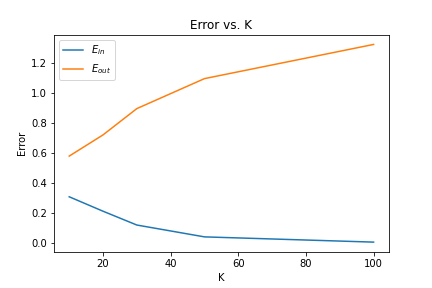
\includegraphics[width=0.7\textwidth]{plots/2d.png}
        \caption{In-sample and out-of-sample error as a function of representation size.}
    \end{center}
    \end{figure}
    As $k$ increases, the in-sample error decreases while the out-of-sample error increases (the model overfits more). This is because the model has more latent factors to better fit the training (in-sample) data, but in doing so overfits the data and causes the out-of-sample error to increase.
\end{solution}

\newpage

\problem[5]
Now, repeat problem D, but this time with the regularization term. Use the following regularization values: $\lambda \in \{10^{-4}, 10^{-3}, 0.01, 0.1, 1\}$. For each regularization value, use the same range of values for $k$ as you did in the previous part. What trends do you notice in the graph? Can you explain them in the context of your plots for the previous part? You should use your code you wrote for part C in 2_notebook.ipynb.

\begin{solution}
    \begin{figure}[H]
    \begin{center}
        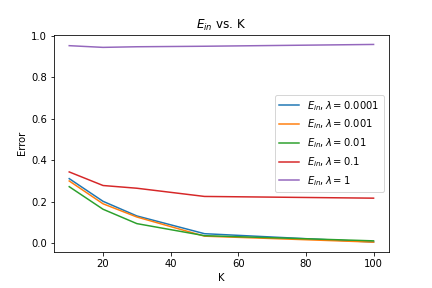
\includegraphics[width=0.7\textwidth]{plots/2e_ein.png}
        \caption{In-sample error for different regularization and $k$}
    \end{center}
    \end{figure}

    \begin{figure}[H]
    \begin{center}
        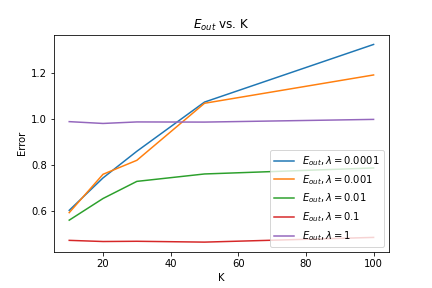
\includegraphics[width=0.7\textwidth]{plots/2e_eout.png}
        \caption{Out-of-sample error for different regularization and $k$}
    \end{center}
    \end{figure}

    Generally, as $k$ increases, as with the last problem, in-sample error decreases and out-of-sample error increases. A higher regularization strength slows the decrease of in-sample-error and decreases the growth of out-of-sample error as $k$ increases, but a too high regularization value results in no additional learning as $k$ increases, with a high in-sample and out-of-sample error ($\lambda = 1$). Thus, the regularization counteracts the overfitting caused by larger $k$, so that the error does not change even as $k$ changes.
\end{solution}






\newpage
\section{Word2Vec Principles [35 Points]}
\materials{Lecture 12}

The Skip--gram model is part of a family of techniques that try to understand language by looking at what words tend to appear near what other words.  The idea is that semantically similar words occur in similar contexts.  This is called ``distributional semantics'', or ``you shall know a word by the company it keeps''.  

The Skip--gram model does this by defining a conditional probability distribution $p(w_O|w_I)$ that gives the probability that, given that we are looking at some word $w_I$ in a line of text, we will see the word $w_O$ nearby.  To encode $p$, the Skip-gram model represents each word in our vocabulary as two vectors in $\mathbb{R}^D$: one vector for when the word is playing the role of $w_I$ (``input''), and one for when it is playing the role of $w_O$ (``output'').  (The reason for the 2 vectors is to help training --- in the end, mostly we'll only care about the $w_I$ vectors.)  Given these vector representations, $p$ is then computed via the familiar softmax function:
\[ p(w_O|w_I) = \frac{\exp \left({v'}_{w_O}^T v_{w_I} \right)}{\sum_{w=1}^W \exp \left( {v_w'}^T v_{w_I} \right)} \tag{2} \label{eqn:softmax} \]
where $v_w$ and $v_w'$ are the ``input'' and ``output'' vector representations of word a $w \in \{1, ..., W\}$.  (We assume all words are encoded as positive integers.)

Given a sequence of training words $w_1, w_2, \hdots, w_T$, the training objective of the Skip-gram model is to maximize the average log probability
\[ \frac{1}{T}  \sum_{t=1}^T \sum_{-s \leq j \leq s, j \neq 0} \log p(w_{t+j}|w_t) \tag{1}\label{eqn:opt} \] where $s$ is the size of the ``training context'' or ``window'' around each word. Larger $s$ results in more training examples and higher accuracy, at the expense of training time.

\newpage

\problem[5]
If we wanted to train this model with naive gradient descent, we'd need to compute all the gradients $\nabla \log p(w_O|w_I)$ for each $w_O$, $w_I$ pair.  How does computing these gradients scale with $W$, the number of words in the vocabulary, and $D$, the dimension of the embedding space? To be specific, what is the time complexity of calculating $\nabla \log p(w_O|w_I)$ for a single $w_O$, $w_I$ pair?

\begin{solution}
    \begin{align*}
        \nabla \log p(w_O|w_I) &= \nabla \log \frac{\exp(v'^T_O v_I)}{\sum_{w=1}^W \exp(v'^T_w v_{w_I})}\\
        &= \nabla \left( v'^T_{w_O} v_{w_I} - \log \sum_{w=1}^W \exp(v'^T_w v_{w_I}) \right)\\
        &= v_{w_I} - \frac{v_{w_I}}{\sum_{w=1}^W \exp(v'^T_w v_{w_I})} \exp{v'^T_w v_{w_I}}
    \end{align*}
    Thus, for each word, the time complexity scales linearly by the dimension of the embedding space, since the dot product (scales linearly with D) must be computed for each word (summation in denominator). Thus, the overall complexity for calculating the gradients for a single pair of words is $O(WD)$.
\end{solution}

\newpage

\problem[10]
When the number of words in the vocabulary $W$ is large, computing the regular softmax can be computationally expensive (note the normalization constant on the bottom of Eq.~\ref{eqn:softmax}). For reference, the standard fastText pre-trained word vectors encode approximately $W \approx 218000$ words in $D=100$ latent dimensions. One trick to get around this is to instead represent the words in a binary tree format and compute the hierarchical softmax.

When the words have all the same frequency, then any balanced binary tree will minimize the average representation length and maximize computational efficiency of the hierarchical softmax. But in practice, words occur with very different frequencies --- words like "a", "the", and "in" will occur many more times than words like "representation" or "normalization".

The original paper (Mikolov et al. 2013) uses a Huffman tree instead of a balanced binary tree to leverage this fact. For the 8 words and their frequencies listed in the table below, build a Huffman tree using the algorithm found \href{https://riptutorial.com/algorithm/example/23995/huffman-coding}{here}.
Then, build a balanced binary tree of depth 3 to store these words. 
Make sure that each word is stored as a \emph{leaf node} in the trees.

The representation length of a word is then the length of the path (the number of edges) from the root to the leaf node corresponding to the word. For each tree you constructed, compute the expected representation length (averaged over the actual frequencies of the words).

\begin{table}[]
\centering
\caption{Words and frequencies for Problem B}
\begin{tabular}{|l|l|}
\hline
Word  & Occurrences \\ \hline
do    & 18          \\
you   & 4           \\
know  & 7           \\
the   & 20          \\
way   & 9          \\
of    & 4           \\
devil & 5           \\
queen & 6           \\ \hline
\end{tabular}
\end{table}

\newpage

\begin{solution}
    \begin{figure}[H]
    \begin{center}
        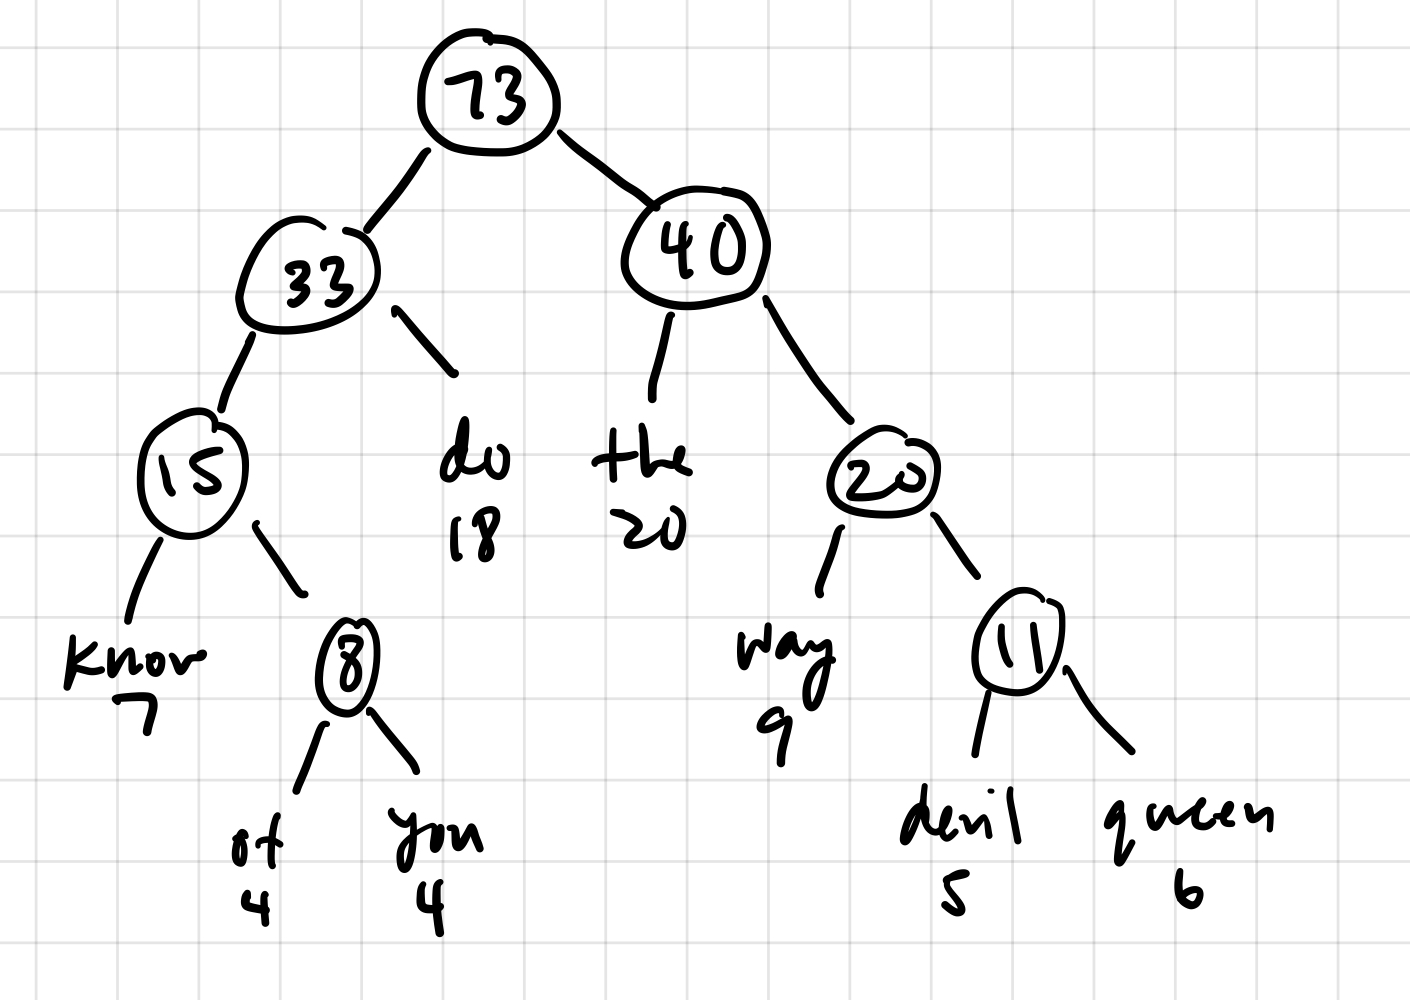
\includegraphics[width=0.7\textwidth]{plots/3b_huffman.jpeg}
        \caption{Huffman tree created using word frequencies.}
    \end{center}
    \end{figure}

    \begin{figure}[H]
    \begin{center}
        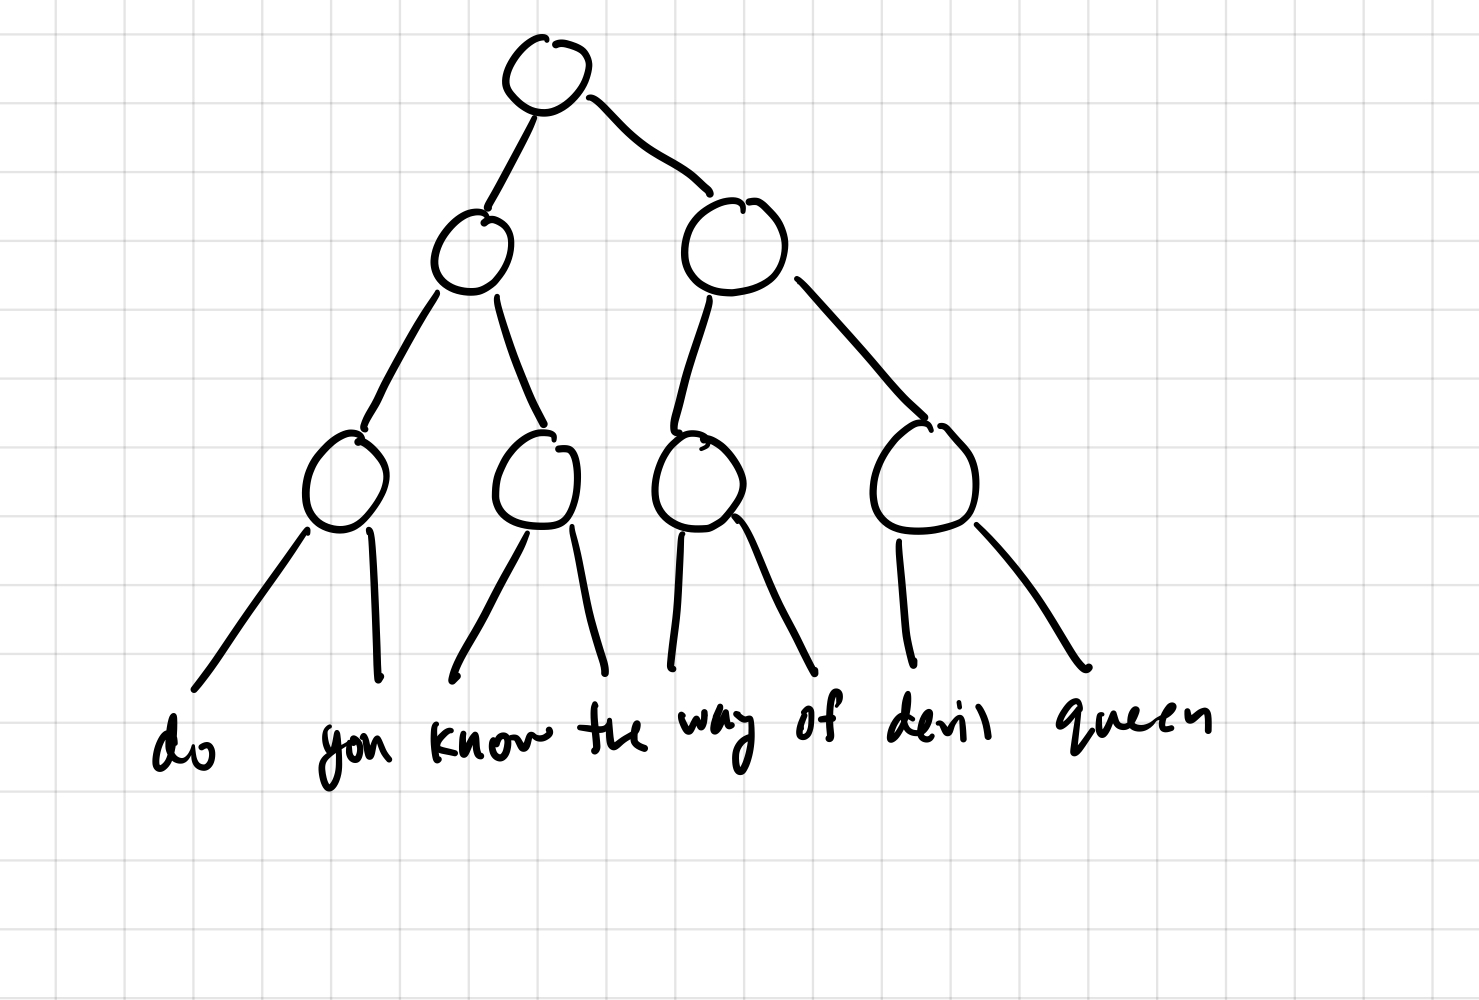
\includegraphics[width=0.7\textwidth]{plots/3b_bbt.jpeg}
        \caption{Balanced binary tree created using words.}
    \end{center}
    \end{figure}
    The expected representation length of the Huffman tree is
    \[
        \frac{1}{73}(2 \cdot 18 + 2 \cdot 20 + 3 \cdot 7 + 3 \cdot 9 + 4 \cdot 4 + 4 \cdot 4 + 4 \cdot 5 + 4 \cdot 6) = \boxed{2.7397}
    \]
    The expected representation length of the balanced binary tree is 3
\end{solution}


\problem[3]
In principle, one could use any $D$ for the dimension of the embedding space.  What do you expect to happen to the value of the training objective as $D$ increases?  Why do you think one might not want to use very large $D$?

\begin{solution}
    The training objective value increases as $D$ increases (less error), since there are more dimensions in the representation for the model to fit, thus lowering error. However, this may not be a good idea since the model could be prone to overfitting as a result.
\end{solution}

\subsection{Implementing Word2Vec}
Word2Vec is an efficient implementation of the Skip--gram model using neural network--inspired training techniques. We'll now implement Word2Vec on text datasets using Pytorch.  This  
\href{http://mccormickml.com/2016/04/19/word2vec-tutorial-the-skip-gram-model/}{blog post} provides an overview of the particular Word2Vec implementation we'll use.

At a high level, we'll do the following:
\begin{enumerate} [(i)]
\item
Load in a list $L$ of the words in a text file

\item
Given a window size $s$, generate up to $2s$ training points for
word $L_i$. The diagram below shows an example of training point generation for $s = 2$:

\begin{figure}[H]
\begin{center}
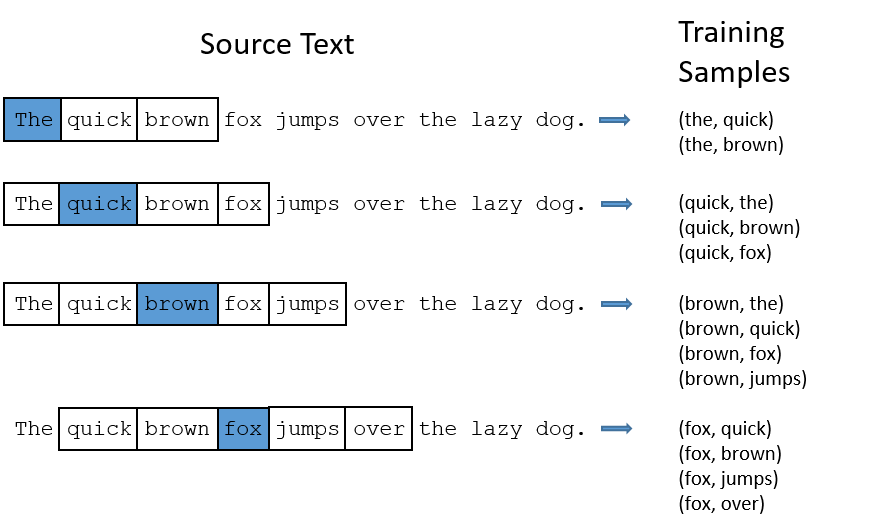
\includegraphics[width=0.7\textwidth]{plots/training_data_example.png}
\caption{Generating Word2Vec Training Points}
\end{center}
\end{figure}


\item
Fit a neural network consisting of a single hidden layer of 10 units on our training data.  The hidden layer should have no activation function, the output layer should have a softmax activation, and the loss function should be the cross entropy function.  

Notice that this is exactly equivalent to the Skip--gram formulation given above where the embedding dimension is 10: the columns (or rows, depending on your convention) of the input--to--hidden weight matrix in our network are the $w_I$ vectors, and those of the hidden--to--output weight matrix are the $w_O$ vectors.

\item
Discard our output layer and use the matrix of weights between our input layer and hidden layer as the matrix of feature representations of our words.

\item
Compute the cosine similarity between each pair of distinct words and determine the top 30 pairs of most-similar words.
\end{enumerate}

\subsubsection{Implementation}

See set5_prob3.ipynb, which implements most of the above.

\newpage

\problem[10]
Fill out the TODOs in the skeleton code; specifically, add code where indicated to train a neural network as described in (iii) above and extract the weight matrix of its input--to--hidden weight matrix. Also, fill out the generate\_traindata() function, which generates our data and label matrices.


\begin{solution}
    \href{https://colab.research.google.com/drive/1_NBkNvw3P_O1XJZFMxLRgxDk9YdC8KkH?usp=sharing}{Code link}

    https://colab.research.google.com/drive/1_NBkNvw3P_O1XJZFMxLRgxDk9YdC8KkH?usp=sharing
\end{solution}

\subsection{Running the code}
Run your model on dr_seuss.txt and answer the following questions:

\problem[2]
What is the dimension of the weight matrix of your hidden layer?

\begin{solution}
    The PyTorch tensor is $10 \times 308$ (however, PyTorch transposes the matrices, so the model really performs multiplication with a $308 \times 10$ matrix).
\end{solution}

\problem[2]
What is the dimension of the weight matrix of your output layer?
\begin{solution}
    The PyTorch tensor is $308 \times 10$. (Again, PyTorch transposes the matrix, so the actual matrix is $10 \times 308$, which matches the hidden layer dimension/output dimension)
\end{solution}

\problem[1]
List the top 30 pairs of most similar words that your model generates.
\begin{solution}
    \begin{itemize}
        \item Pair(or, anywhere), Similarity: 0.99958247
        \item Pair(anywhere, or), Similarity: 0.99958247
        \item Pair(eggs, ham), Similarity: 0.9990665
        \item Pair(ham, eggs), Similarity: 0.9990665
        \item Pair(do, them), Similarity: 0.9983842
        \item Pair(them, do), Similarity: 0.9983842
        \item Pair(star, lot), Similarity: 0.9981338
        \item Pair(lot, star), Similarity: 0.9981338
        \item Pair(car, train), Similarity: 0.99767697
        \item Pair(train, car), Similarity: 0.99767697
        \item Pair(am, sam), Similarity: 0.9976195
        \item Pair(sam, am), Similarity: 0.9976195
        \item Pair(dish, sam), Similarity: 0.99745214
        \item Pair(hop, am), Similarity: 0.9972182
        \item Pair(wish, hop), Similarity: 0.9971074
        \item Pair(go, gox), Similarity: 0.99676085
        \item Pair(gox, go), Similarity: 0.99676085
        \item Pair(long, way), Similarity: 0.996485
        \item Pair(way, long), Similarity: 0.996485
        \item Pair(book, read), Similarity: 0.9962874
        \item Pair(read, book), Similarity: 0.9962874
        \item Pair(dog, cat), Similarity: 0.9962772
        \item Pair(cat, dog), Similarity: 0.9962772
        \item Pair(another, today), Similarity: 0.99608654
        \item Pair(today, another), Similarity: 0.99608654
        \item Pair(two, home), Similarity: 0.99598694
        \item Pair(home, two), Similarity: 0.99598694
        \item Pair(no, shoe), Similarity: 0.99592084
        \item Pair(shoe, no), Similarity: 0.99592084
        \item Pair(be, gox), Similarity: 0.9954331
    \end{itemize}
    
\end{solution}

\newpage

\problem[2]
What patterns do you notice across the resulting pairs of words?
\begin{solution}
    Most words that are frequently used near each other (``green eggs and ham'') have a high similarity score. Additionally, due to the symmetry in the generation of x,y pairs, the two orderings of a pair of words are similar to each other in similarity score.
\end{solution}

\end{document}

